\documentclass[../TinyBot.tex]{subfiles}
\begin{document}
    
\section{Motor} \label{sec:motor}
% gearbox, motor

To follow this guide it is not necessary to have an understanding of how motors work, though it may be interesting for you to learn. \href{https://www.explainthatstuff.com/electricmotors.html}{This} link has a good indepth explanation. 

\bigskip


Motors turn in proportion to the amount of current put through them. More current means a faster motor. 
When a motor stalls, it stops rotating. This happens when there is more force acting on the motor shaft than the motor can overcome. The stall current of a motor is the maximum current drawn when a motor stalls, in other words, applying its maximum torque - known as stall torque. \\

Similarly, free current is the current drawn when the motor is rotating freely, under no load - free current can also be thought of as the amount of current that has to be applied for a motor to overcome its internal friction. The stall current is usually much larger than the free current, and keeping a motor in a stalled condition can lead to overheating and damage to the motor due to the high current through it. The relationships between current, speed, and torque can be seen in Figure \ref{fig:motor:stats}.

\begin{figure}[h!]
    \centering
    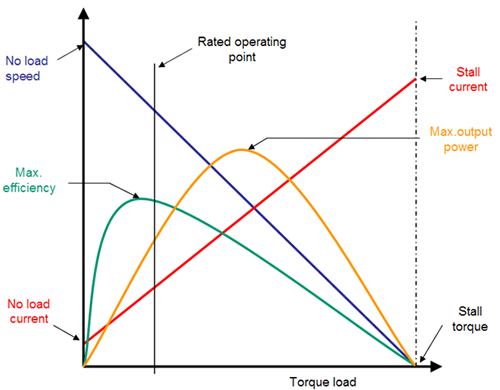
\includegraphics[width=0.6\textwidth]{motor-stats.jpg}
    \caption{Motor characteristics plot}
    \label{fig:motor:stats}
\end{figure}

\bigskip



Each motor has a certain amount of torque it can provide, which depends greatly on the size and current draw of the motor. The speed of a motor also depends on the current going through the motor. Motor torque and speed are proportional, with torque increasing as speed decreases. This is because the mechanical power of a motor depends on torque $\times$ speed ($P=\tau \omega$), the power of a motor is constant meaning that when $\tau$ increases, $\omega$ must decrease. 
\bigskip

It is possible to control the speed of a motor by controlling the input voltage, however this often results in high speeds and low torques. When we want to use motors to drive a robot around we're going to need relatively high torque from our motors as we need to overcome friction between the robot's wheels and the ground. To increase the torque of a motor, we want to use a gearbox. \\


Gearboxes chain together different sized gears (gear size is commonly measured by the number of teeth on the gear which leads to a larger diameter), with the ratio of teeth size determining the output speed/torque. The ratio can be calculated as 


% A gear box is useful for controlling the speed and torque outputs for motors. A motor has a maximum torque it can operate at before it starts to fail, this is known as a stall torque. If you want to increase the stall torque, you will need to lower the output speed, which can be accomplished with a gear box. The important factors to consider are the number of teeth of the gears for the input and output gears. The torque and speed are inversely proportional. The value of these ratios compared can be calculated as follows.\\
    
\[ R = \frac{N_1}{N_1} = \frac{D_1}{D_1} = \frac{\omega_2}{\omega_1} \]
\bigskip

\begin{wrapfigure}{r}{0.4\textwidth}
    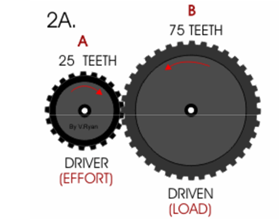
\includegraphics[width=0.4\textwidth]{gear_labelled.png}
        \captionof{figure}{Driver and Driven Gear}
        \label{fig:gear-driver-driven}
\end{wrapfigure}

In the above equation, $\omega$ is the angular velocity, $D$ is the diameter of the gear, and $N$ is the number of teeth. \\

The ratio can be expressed in plain English as a higher number of teeth meaning a smaller angular velocity and a larger diameter gear. This makes sense intuitively, in Figure \ref{fig:gear-driver-driven} gear A has 1/3 the number of teeth of gear B. This means that gear A will fully rotate 3 times in the time it takes gear B to rotate once. The gears must be rotating at the same angular velocty as they are mechanically linked via the gear teeth, and to maintain power (as no energy can be destroyed) gear B must have more torque than gear A. 


\bigskip

We can take advantage of this to increase the output torque of a gearbox to whatever torque we need by simply changing the gear ratios within a gearbox. For the size of motor and gearbox required for TinyBot, it is standard to find the gearbox attached to the motor and so the gear ratio cannot be changed. For larger (higher power) motors, the gearbox is usually a distinct component which can be customised according to the specific speed/torque requirements of the application. \\

It is possible to buy both geared and non-geared motors. It is usually easy to spot when a motor has a gearbox attached, as there will be an additional shape attached to the base motor as shown in the images below. 

% TODO: images of geared and non geared motors. For this project, make sure you have a geared motor - non-geared motors will not be able to supply enough torque for your robot to move. 

\begin{figure}[h!]
    \centering
    \begin{subfigure}[t]{0.3\textwidth}
        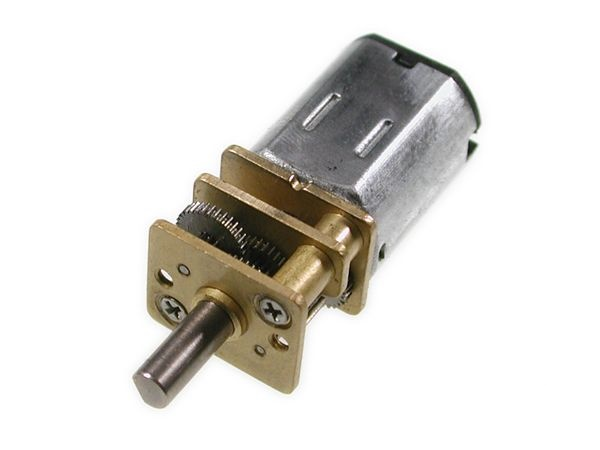
\includegraphics[width=\textwidth]{gearedmotor1.jpg}
        \caption{A Geared Motor}
    \end{subfigure}
    \begin{subfigure}[t]{0.3\textwidth}
        \centering
        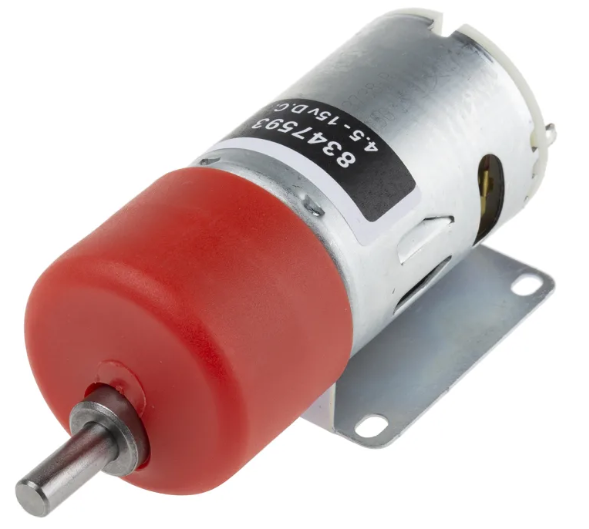
\includegraphics[width=0.8\textwidth]{gearedmotor2.png}
        \caption{A Geared Motor}
    \end{subfigure}
    \begin{subfigure}[t]{0.3\textwidth}
        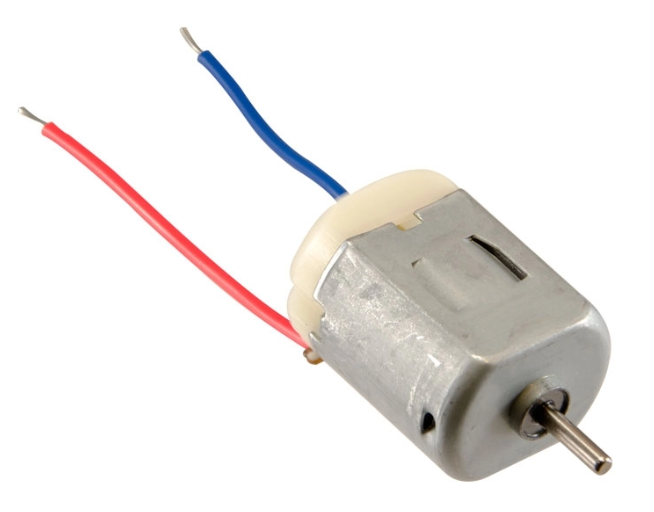
\includegraphics[width=\textwidth]{gearedmotornot.png}
        \caption{Not a Geared Motor}
    \end{subfigure}
\end{figure}


% When connecting multiple gears, we call this a gear train. There are two types of gear trains, simple and complex. Simple gear trains are much like their name, simple. They connect next to each other and you only need to do the calculation for the first gear as an input gear and last gear as the output gear. These are useful for rapidly increasing torque or speed. Compound gear trains are slightly different and require a bit more thinking. A compound gear train means there can be multiple gears on the same shaft, meaning the gear ratio of the entire system will need to be calculated with each connecting gear and transfer the ratios through each individual shaft. You won’t have to deal with compound gear trains for this project, but feel free to investigate it more.
% To summarise gears, the ratio of your input gear to output gear affects the characteristics of your output performance. If you want a higher torque use a larger output gear. If you want more speed, use a smaller output gear.

% \begin{figure}[h]
%     \centering
%     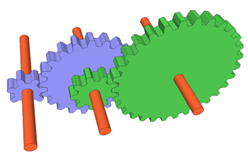
\includegraphics{compound_gears.png}
%     \label{fig:gear-complex}
%     \caption{Complex Gear Train}
% \end{figure}


\end{document}